\documentclass[12pt,a4paper]{article}

% Packages for formatting
\usepackage[margin=1in]{geometry}
\usepackage{multicol}
\usepackage{amsmath,amssymb}
\usepackage{array}
\usepackage{fancyhdr}
\usepackage{setspace}
\usepackage{tikz}

\pagestyle{fancy}
\fancyhf{}
\lhead{Year 7 Arithmetic Revision}
\rhead{Page \thepage}
\setlength{\parindent}{0pt}
\setstretch{1.2}

\begin{document}

\begin{center}
    \vspace{2em}
    {\LARGE \textbf{Four Operations Revision Worksheet}} \\[0.5em]
    \vspace{1em}
    \textbf{Whole Numbers, Decimals, and Negative Numbers} \\[0.5em]
    \vspace{1em}
 \end{center}

\hrule
\vspace{1em}

\section*{Section 1: Addition and Subtraction}

\textbf{Remember:} Line up the decimal points carefully. When working with negatives, think about the sign!

\begin{multicols}{2}
\begin{enumerate}
    \item $45 + 376 =$
    \vspace{2em}
    \item $328.5 + 19.47 =$
    \vspace{2em}
    \item $7.63 + (-2.8) =$
    \vspace{2em}
    \item $-12 + 7 =$
    \vspace{2em}
    \item $56.3 - 18.72 =$
    \vspace{2em}
    \item $-4 - (-9) =$
\end{enumerate}
\end{multicols}


\section*{Section 2: Multiplication}

\textbf{Remember:} 
\begin{itemize}
    \item Count the signs: an \textbf{even} number of negatives gives a positive answer, an \textbf{odd} number gives a negative answer.
    \item We need to be careful when multiplying decimals, and keep track of the decimal point, three methods are described below.
\end{itemize}


For the example multiplication: $3.4 \times 1.2$, the three options are:

\subsection*{1. Factoring Up to Whole Numbers}


We can make both numbers whole by multiplying by powers of 10. These are $10$, $100$, $1\,000$, $10\,000$, \dots \quad etc.

Multiply \(3.4\) by \(10\) to make it \(34\).  
Multiply \(1.2\) by \(10\) to make it \(12\).

Now we have:
\[
34 \times 12 = 408
\]

But we multiplied the numbers by \(10 \times 10 = 100\),  
so we divide the answer by \(100\):

\[
\frac{408}{100} = 4.08
\]

---

\subsection*{2. Counting Decimal Places}

\begin{enumerate}
    \item Multiply the numbers as if there are no decimal points.  
    \item Count how many decimal places there are in total in the question.  
    \item Put that many decimal places back into your answer.
\end{enumerate}

\textbf{Example:} \(3.4 \times 1.2\)

Ignore the decimals: \(34 \times 12 = 408\)

There is \textbf{1 decimal place} in 3.4 and \textbf{1} in 1.2, so \textbf{2 in total.}

\vspace{1em}

So the answer is \(4.08\) 

---

\subsection*{3. Lattice Method with Decimal Alignment}

You can use the lattice method to track the decimal points too.

\begin{center}
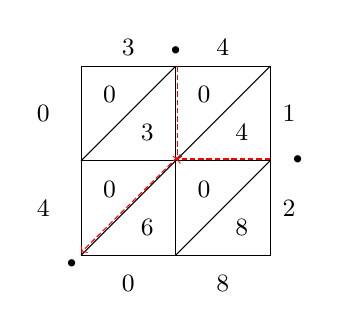
\begin{tikzpicture}[scale=1.2, every node/.style={font=\small}]

% Grid (2x2 for digits 3,4 × 1,2)
\draw (0,0) rectangle (2,2);
\draw (1,0) -- (1,2);
\draw (0,1) -- (2,1);


\draw (0,0) -- (2,2);
\draw (1,0) -- (2,1);
\draw (0,1) -- (1,2);


% Top numbers (3 and 4)
\node at (0.5,2.2) {3};
\node at (1.5,2.2) {4};

% Side numbers (1 and 2)
\node at (2.2,1.5) {1};
\node at (2.2,0.5) {2};

% Products in cells (tens and ones separated)
% 3×1 = 3, 4×1 = 4, 3×2=6, 4×2=8
\node at (0.3,1.7) {0};
\node at (0.7,1.3) {3};

\node at (1.3,1.7) {0};
\node at (1.7,1.3) {4};

\node at (0.3,0.7) {0};
\node at (0.7,0.3) {6};

\node at (1.3,0.7) {0};
\node at (1.7,0.3) {8};

% Diagonal sums
\node at (1.5,-0.3) {8};
\node at (0.5,-0.3) {0};
\node at (-0.4,0.5) {4};
\node at (-0.4,1.5) {0};

% Decimal point placement
\node at (2.3,1) {\Huge$\cdot$};
\node at (1, 2.15) {\Huge$\cdot$};

% decimal point movement to result

\draw[red, dash pattern=on 2pt off 1pt, ->] (1.02,2.0) -- (1.02,1);
\draw[red, dash pattern=on 2pt off 1pt, ->] (2,1.02) -- (1,1.02);
\draw[red, dash pattern=on 2pt off 1pt, ->] (1.02,1.04) -- (0,0.03);

\node at (-0.1,-0.1) {\Huge$\cdot$};

\end{tikzpicture}

\end{center}


Find where the decimal points in each number meet, then follow the diagonal down to the left, that will be where the decimal point is in the answer.

\vspace{1em}

In the example above we get \(4.08\), the same as before!

---

\vspace{2em}

Now try these questions:

\begin{center}
\begin{tabular}{p{0.28\textwidth} p{0.28\textwidth} p{0.28\textwidth}}
1. $24 \times 6 =$ \vspace{2em} & 
5. $3.4 \times 1.2 =$ \vspace{2em} & 
9. $-3 \times 4 =$ \vspace{2em} \\

2. $-2 \times -3 \times -2 =$ \vspace{2em} & 
6. $5.6 \times (-0.3) =$ \vspace{2em} & 
10. $0.0034 \times 68.7 =$ \vspace{2em} \\

3. $0.25 \times 0.4 =$ \vspace{2em} & 
7. $12.5 \times 0.08 =$ \vspace{2em} & 
11. $-4.2 \times 0.5 \times -0.5 =$  \vspace{2em} \\

4. $1.2 \times 0.06 =$ \vspace{2em} & 
8. $0.09 \times 0.7 =$ \vspace{2em} & 
12. $-0.6 \times -0.3 \times -2 =$ \vspace{2em} \\
\end{tabular}
\end{center}



\newpage

\section*{Section 3: Division}

\textbf{Remember:}
\begin{itemize}
    \item Use the bus stop method unless you can do it in your head.
    \item If the divisor is a decimal, you need to make it a whole  number (remember to apply the factor to both numbers!): \newline $ 66 \div 0.33 = 6600 \div 33 = 200 $
    \item Chunk larger divisors into smaller factors if helpful. \newline $176 \div 16 = ( 176 \div 4) \div 4 = 44 \div 4 = 11$
\end{itemize}

\begin{center}
\textbf{Division Practice}
\end{center}

\begin{center}
\begin{minipage}[t]{0.3\textwidth}
\vspace{0.5em}
\begin{enumerate}
    \item $84 \div 7 =$ \vspace{1em}
    \item $156 \div 12 =$ \\[0.3em]
    \textit{(Try chunking!)} \vspace{1em}
    \item $48 \div (-6) =$ \vspace{1em}
    \item $4.8 \div 0.4 =$ \vspace{1em}
\end{enumerate}
\end{minipage}
\hfill
\begin{minipage}[t]{0.3\textwidth}  
\begin{enumerate}\setcounter{enumi}{4}
    \item $-9 \div -3 =$ \vspace{1em}
    \item $8280 \div 24 =$ \vspace{1em}
    \item $3.6 \div 0.6 =$ \vspace{1em}
    \item $0.84 \div 0.07 =$ \vspace{1em}
    \item $7.2 \div 0.6 =$
\end{enumerate}
\end{minipage}
\hfill
\begin{minipage}[t]{0.3\textwidth}
\begin{enumerate}\setcounter{enumi}{9}
    \item $-12.6 \div 0.3 =$ \vspace{1em}
    \item $0.56 \div 0.08 =$ \vspace{1em}
    \item $6.4 \div (-0.2) =$ \vspace{1em}
    \item $-1.8 \div 0.3 =$ \vspace{1em}
    \item $-0.45 \div 0.05 =$
\end{enumerate}
\end{minipage}
\end{center}

\vspace{1em}
\hrule
\vspace{1em}


\section*{Section 4: Mixed Practice}

\textbf{Challenge yourself!} Decide which methods to use.

\begin{multicols}{1}
\begin{enumerate}
\item $12.5 + (-3.4) =$ \
\vspace{1em}
\item $-3 \times 4 \times -2 =$ \
\vspace{1em}
\item $24 \div (-6) + 5 \times 2 =$ \
\vspace{1em}
\item $6.3 \div 0.3 =$ \
\vspace{1em}
\item $(-2.4 \times 3.5) \div -0.7 =$ \
\vspace{1em}
\item $-15 + 28.4 \div 4 =$ \
\vspace{1em}
\item $7.25 - 3.68 =$ \
\vspace{1em}
\item $-8 \times (5 - 7) =$ \
\vspace{1em}
\item $9.6 \div 1.2 + (-3) \times 2 =$ \
\vspace{1em}
\item $-36 \div (-9) =$ \
\vspace{1em}
\end{enumerate}
\end{multicols}

\section*{Extension Word Problems}

\begin{enumerate}
    \item The temperature was $-3^\circ$C and dropped by $5^\circ$C overnight. What is the new temperature?
    \vspace{2em}
    \item A scuba diver descends $2.5$ m per minute for 4 minutes, then ascends $3$ m. What is the diver’s final depth?
    \vspace{2em}
    \item A submarine starts at sea level and travels vertically $-4.2$ km, then another $-3.8$ km. How far is it from the surface now? What is the submarine's altitude?
    \vspace{2em}
    \item Some numbers produce recurring decimals when used as divisors. Find the decimal result of 1 divided by each of the first 7 prime numbers. Some results terminate while others recur. Can you explain why?
\end{enumerate}

\end{document}
